\documentclass[pdflatex,compress,mathserif]{beamer}

%\usetheme[dark,framenumber,totalframenumber]{ElektroITK}
\usetheme[darktitle,framenumber,totalframenumber]{ElektroITK}

\usepackage[utf8]{inputenc}
\usepackage[T1]{fontenc}
\usepackage{lmodern}
\usepackage[bahasai]{babel}
\usepackage{amsmath}
\usepackage{amsfonts}
\usepackage{amssymb}
\usepackage{graphicx}
\usepackage{multicol}

\newcommand*{\Scale}[2][4]{\scalebox{#1}{$#2$}}%

\title{PEMODELAN JARINGAN KOMUNIKASI}
\subtitle{Connectivity Troubleshooting}

\author{Tim Dosen Pengampu}

\begin{document}
	
\maketitle

\section{IGP Interior Gateway Protocol Fundamentals}

\begin{frame}
	\frametitle{RIP Characteristics}
	\begin{itemize}
		\item The Routing Information Protocol (RIP) is a Distance Vector
routing protocol
		\item It uses hop count as its metric
		\item The maximum hop count is 15
		\item It will perform Equal Cost Multi Path, for up to 4 paths by default
	\end{itemize}
\end{frame}

\begin{frame}
	\frametitle{RIPv2 vs RIPv1}
	\begin{itemize}
		\item RIPv1 is a legacy protocol which is not typically used anymore
(although it is still supported on Cisco routers)
		\item RIPv1 does not send subnet mask information with routing
updates so Variable Length Subnet Masking (VLSM) is not
supported. RIPv2 does support VLSM.
		\item RIPv1 updates are sent every 30 seconds as broadcast traffic.
RIPv2 uses multicast address 224.0.0.9
		\item RIPv2 supports authentication, RIPv1 does not.
	\end{itemize}
\end{frame}

\begin{frame}
	\frametitle{RIPng}
	\begin{itemize}
		\item RIPng (RIP next generation) supports IPv6 networks
		\item It is not covered on the CCNA exam
	\end{itemize}
\end{frame}

\begin{frame}
	\frametitle{RIPv2 Configuration}
	\begin{figure}
		\centering
		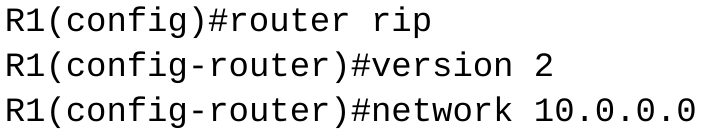
\includegraphics[width=0.7\linewidth]{img/img01}
	\end{figure}
	\begin{itemize}
		\item The ‘network’ command should reference a classful network. No subnet
		mask is specified.
	\end{itemize}
\end{frame}

\begin{frame}
	\frametitle{Auto-Summary}
	\begin{itemize}
		\item RIP will automatically summarise routes to the classful boundary by
default
		\item For example, 192.168.10.1/30 will be advertised as 192.168.10.0/24
		\item 172.16.10.1/30 will be advertised as 172.16.0.0/16
		\item This is almost never desirable
	\end{itemize}
	\begin{figure}
		\centering
		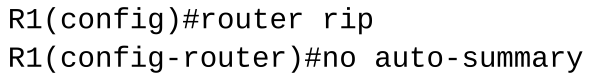
\includegraphics[width=0.7\linewidth]{img/img02}
	\end{figure}
\end{frame}

\begin{frame}
	\frametitle{Manual Summarization}
	\begin{itemize}
		\item Manual summarisation gives you control of exactly how you summarise
		\item The individual summarised routes are not advertised - only their summary
route
	\end{itemize}
	\begin{figure}
		\centering
		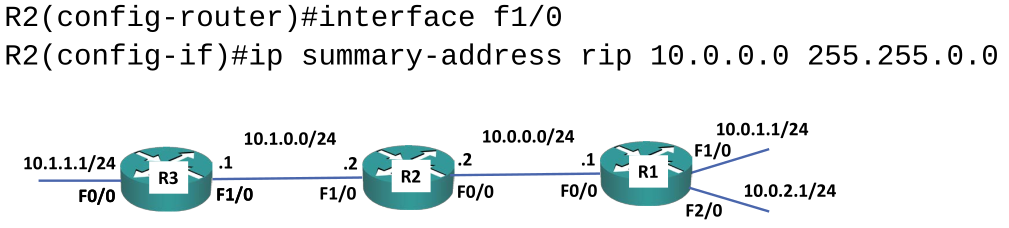
\includegraphics[width=\linewidth]{img/img03}
	\end{figure}
\end{frame}

\begin{frame}
	\frametitle{RIPv2 Verification – \\show ip protocols}
	\begin{figure}
		\centering
		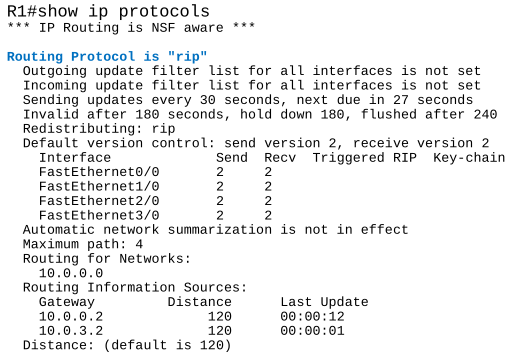
\includegraphics[width=0.8\linewidth]{img/img04}
	\end{figure}
\end{frame}

\begin{frame}
	\frametitle{RIPv2 Verification – \\show run | section rip}
	\begin{figure}
		\centering
		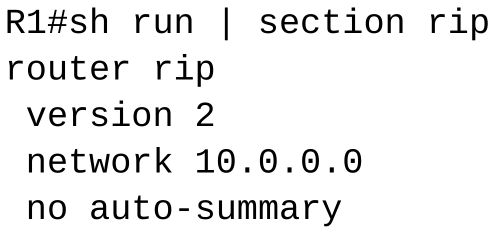
\includegraphics[width=0.8\linewidth]{img/img05}
	\end{figure}
\end{frame}

\begin{frame}
	\frametitle{RIPv2 Verification – \\show ip route}
	\begin{figure}
		\centering
		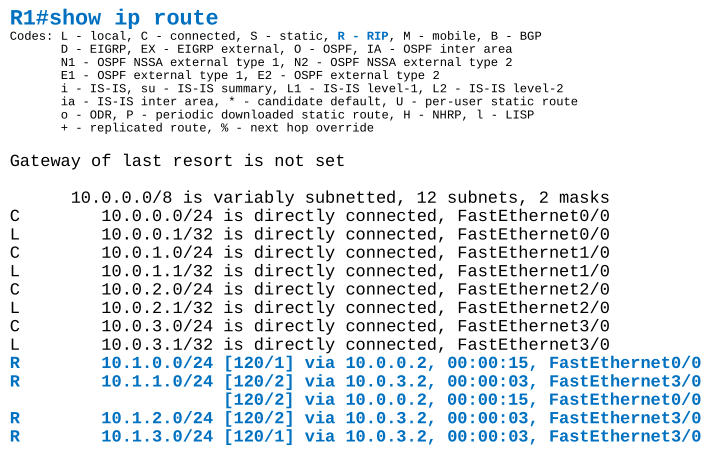
\includegraphics[width=0.8\linewidth]{img/img06}
	\end{figure}
\end{frame}

\begin{frame}
	\frametitle{RIPv2 Verification – \\show ip rip database}
	\begin{figure}
		\centering
		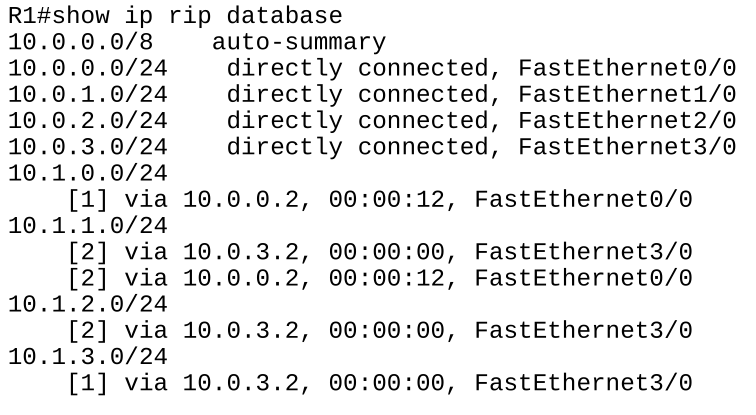
\includegraphics[width=0.8\linewidth]{img/img07}
	\end{figure}
\end{frame}

\begin{frame}
	\frametitle{Default Route Injection}
	\begin{figure}
		\centering
		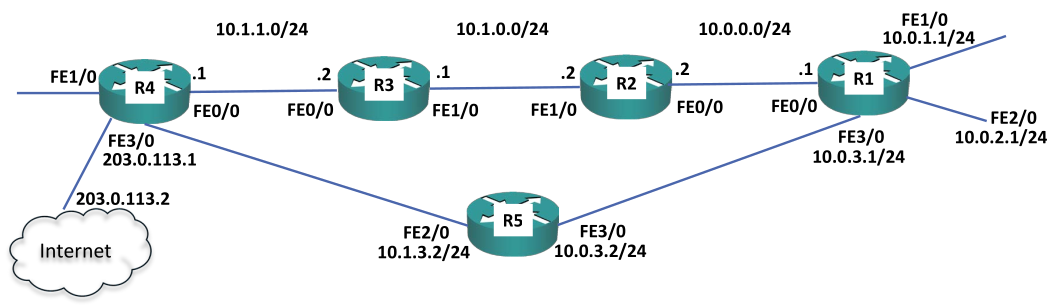
\includegraphics[width=\linewidth]{img/img08}
	\end{figure}
\end{frame}

\begin{frame}
	\frametitle{Default Route Injection}
	\begin{figure}
		\centering
		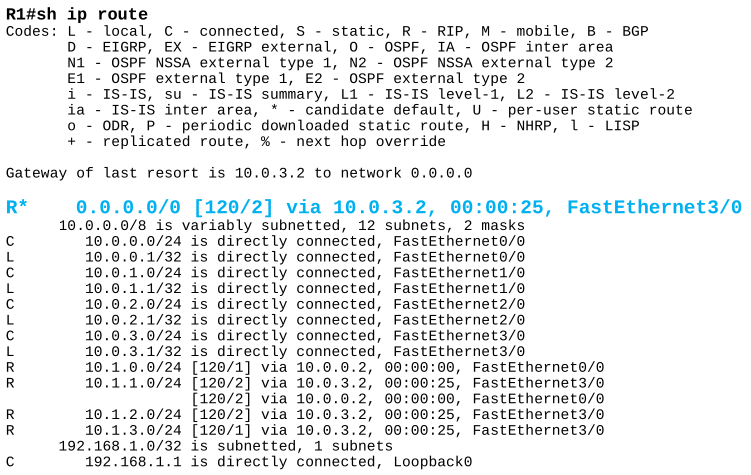
\includegraphics[width=\linewidth]{img/img09}
	\end{figure}
\end{frame}

\section{EIGRP - the Enhanced Interior Gateway Routing Protocol}

\section{EIGRP Lab Demo}

\end{document}